
\chapter{Methodology}
This chapter is organized as follows: Section \ref{sec:topic_modeling_method} will discuss the concept of Topic Modeling, Section \ref{sec:llm_method} will discuss the concept of Large Language Models, and finally Section \ref{sec:code_setup} will discuss how to implement this in Julia programming language.
\section{Morphological Analysis}
This section will discuss the statistical analyses of the morphology of Qur'\=an's texts. In particular, the focus would be on the parts of speech of the Qur'\=an.
\section{Rhythmic Analysis}
As discussed in Chapter \ref{ch:introduction}, one of the Qur'\=an's characteristics is the rhythmic feature of the \arb[trans]{'ayaT} \arb{'ayaT} in the \arb[trans]{sUraT}. This can be easily confirmed by simply learning the phonetical alphabets of Arabic, and reciting through the \arb[trans]{'ayaT} \arb{'ayaT} of the Qur'\=an. However, none has ever studied this rhythmic feature objectively from a statistical perspective. In this section, the methodology on how to analyze this is discussed. To start with, consider the following example:
\begin{exmp}
    Table \ref{tbl:surah_alfatihah} shows the verses of the first chapter of the Qur'\=an, \arb[trans]{sUraTu 'l-fAti.haT} \arb{sUraTu 'l-fAti.haT}. In this table the last two syllables are highlighted in red. In Arabic, when the sentence ends or there is a pause, the last vowel of the syllable is silent, that is, not pronounced. So that, for the first \arb[trans]{'ayaT} \arb{'ayaT}, the last two syllables is read as \arb[trans]{hImi} \arb{hImi}, but because this is the end of the said \arb[trans]{'ayaT} \arb{'ayaT}, then it is read as \arb[trans]{hIm} \arb{hIm}. This is the same case with the remaining six \arb[trans]{'ayaT} \arb{'ayaT}. Therefore, following the said rule, the \arb[trans]{'ayaT} \arb{'ayaT} of \arb[trans]{sUraTu 'l-fAti.haT} \arb{sUraTu 'l-fAti.haT} are: \arb[trans]{hIm} \arb{hIm}, \arb[trans]{mIn} \arb{mIn}, \arb[trans]{hIm} \arb{hIm}, \arb[trans]{dIn} \arb{dIn}, \arb[trans]{`in} \arb{`in}, \arb[trans]{qIm} \arb{qIm}, and \arb[trans]{lIn} \arb{lIn}. As observed, all of the ending syllables has a vowel of \textit{i}, and this consistency is what produces the rhyme. In this paper, the rhymes across all \arb[trans]{'Ayat} of the Qur'\=an are studied.\\
    \begin{table}
        \caption{The verses or \arb[trans]{'Ayat} \arb{'Ayat} of \arb[trans]{sUraTu 'l-fAti.haT} \arb{sUraTu 'l-fAti.haT}}
        \begin{tabularx}{\textwidth}{XX}
            \toprule
            \textbf{Transliteration}&\textbf{Verses} or \arb[trans]{'Ayat} \arb{'Ayat}\\
            \midrule
            \arb[trans]{bismi 'l-lahi 'l-ra.hmAni 'l-ra\arbcolor[red]{hIm}i ((1))}&
            \arb[fullvoc]{bismi 'l-lahi 'l-ra.hmAni 'l-ra\arbcolor[red]{hImi} ((1))}
            \\[0.4cm]
            \arb[trans]{'l.hamdu lillahi rabbi 'l`Ala\arbcolor[red]{mIn}a ((2))}&
            \arb[fullvoc]{'l-.hamdu lillahi rabbi 'l-`Ala\arbcolor[red]{mIna} ((2))}\\[0.4cm]
            
            \arb[trans]{'l-ra.hmAni 'l-ra\arbcolor[red]{hIm}i ((3))}&
            \arb[fullvoc]{'l-ra.hmAni 'l-ra\arbcolor[red]{hImi} ((3))}\\[0.4cm]
            
            \arb[trans]{mAliki yawmi 'l-\arbcolor[red]{dIn}i ((4))}&
            \arb[fullvoc]{mAliki yawmi 'l-\arbcolor[red]{dIni} ((4))}\\[0.4cm]
            
            \arb[trans]{'iyyAka na`budu wa-'iyyaka nasta\arbcolor[red]{`In}u ((5))}&
            \arb[fullvoc]{'iyyAka na`budu wa-'iyyaka nasta\arbcolor[red]{`Inu} ((5))}\\[0.4cm]
            
            \arb[trans]{'ihdinA 'l-.sirA.ta 'l-musta\arbcolor[red]{qIm}a ((6))}&
            \arb[fullvoc]{'ihdinA 'l-.sirA.ta 'l-musta\arbcolor[red]{qIma} ((6))}\\[0.4cm]

            \arb[trans]{.sirA.ta 'lla_dIna 'an`amta `alayhim .gayri 'l-ma.g.dUbi `alayhim wa-lA 'l-.dAl\arbcolor[red]{lIn}a ((7))}&
            \arb[fullvoc]{.sirA.ta 'lla_dIna 'an`amta `alayhim .gayri 'l-ma.g.dUbi `alayhim wa-lA 'l-.dA\arbcolor[red]{llIna} ((7))}\\[0.4cm]
            \bottomrule
        \end{tabularx}
        \label{tbl:surah_alfatihah}
    \end{table}
\end{exmp}

The first method for studying the rhyme is to simply visualize this through a line chart, with the x-axis being the \arb[trans]{'ayaT} \arb{'ayaT} number and the y-axis being the last syllables. The idea then is to understand the pattern of how the vowels switch. Figure \ref{fig:fatihah_baqarah_rhythmic_method} shows the rhythmic pattern of the last pronounced syllable of both \arb[trans]{sUraTu 'l-fati.haT} \arb{sUraTu 'l-fati.haT} and \arb[trans]{sUraTu 'l-baqaraT} \arb{sUraTu 'l-baqaraT}.

\begin{figure}[!t]
    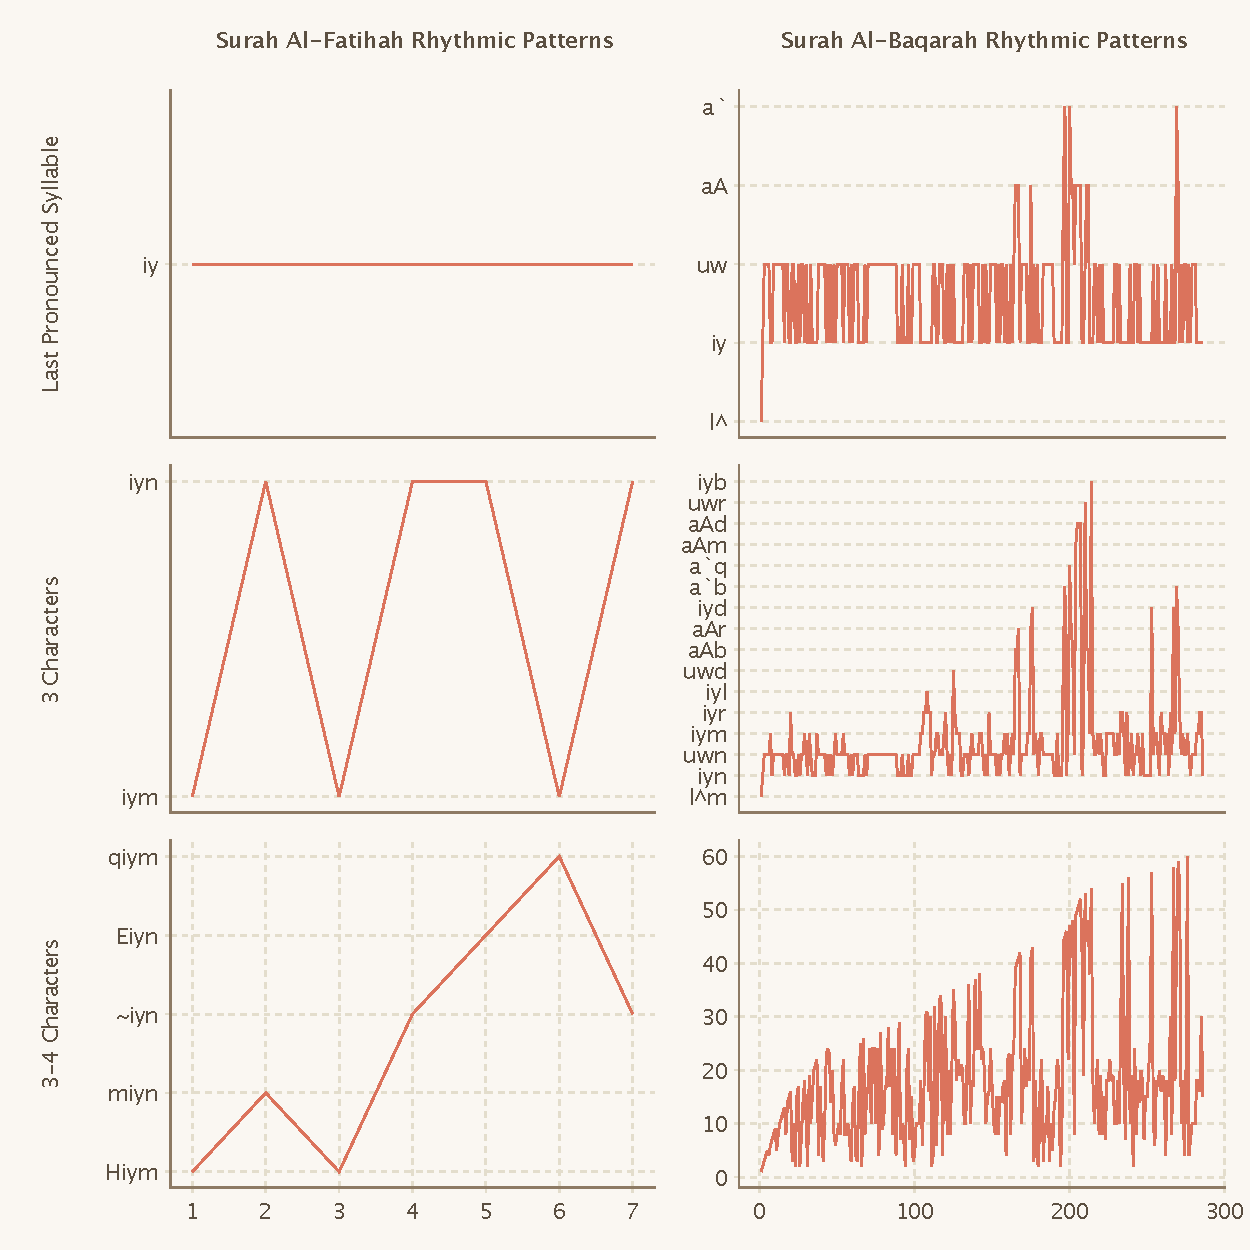
\includegraphics[width=\textwidth]{img/plot_rhythmic1.pdf}
    \caption{Rhythmic pattern of the last pronounced syllables of the \arb[trans]{sUraTu 'l-fati.haT} \arb{sUraTu 'l-fati.haT} and \arb[trans]{sUraTu 'l-baqaraT} \arb{sUraTu 'l-baqaraT}}
    \label{fig:fatihah_baqarah_rhythmic_method}
\end{figure}

With the data given in Figure \ref{fig:fatihah_baqarah_rhythmic_method}, we want to study if there are some interesting patterns on the switch of the rhythm, like in terms of topic, does the switch to particular rhythmic syllables imply a change in topic being discussed in the \arb[trans]{sUraT} \arb{sUraT}? Further, we also would want to model the dynamic of the changes using a statistical model. The first one is a non-dynamic model and is called Bayesian Networks model, and then the other one accounts the changes over the \arb[trans]{'ayaT} \arb{'ayaT} numbers, and this model is called the Discrete-Time Markov Models, both discussed in the succeeding sections after the concept of Graphical models, which is the basis of the said model.
\subsection{Directed Probabilistic Graphical Models (PGM)}
Probabilistic graphical models or simply graphical models are probability models represented graphically using nodes as random variables and segments or links as dependencies between variables. The link between the nodes is expressed as a chain rule of a conditional probability.

\begin{exmp}\label{exmp:directgraph}
Figure \ref{fig:baysnet} (a) illustrates the connections between three variables. The joint probability distribution of these random variables is expressed as follows:
$$
p(X_1,X_2,X_3)=p(X_1)p(X_2|X_1)p(X_3|X_1,X_2).
$$
On the other hand, Figure \ref{fig:baysnet} (b) has $N$ events namely $X_1,X_2,\cdots, X_N$, such that the joint probability is given by
$$
\begin{aligned}
p(X_1,X_2,\cdots,X_N)&=p(X_1)p(X_2)p(X_3|X_1,X_2)\cdots p(X_n|X_1,X_2)\\
&= p(X_1) p(X_2)\prod_{n=3}^{N} p(X_n|X_1,X_2).
\end{aligned}
$$
\end{exmp}
\begin{figure}
\begin{minipage}[c]{\textwidth}\centering
\begin{subfigure}[b]{.5\textwidth}
\centering
\begin{tikzpicture}[>=latex,auto,thick,node distance = 3cm]
\tikzstyle{every state}=[fill=white,draw=black,thick,text=black,scale=1]
\node[state] (A)  {$X_1$};
\node[state] (B) [above right of = A] {$X_2$};
\node[state] (C) [below right of = B] {$X_3$};
\path[->]
  (A) edge (B)
  (B) edge (C)
  (A) edge (C);
\end{tikzpicture}
\subcaption{Directed Acyclic Graph.}
\end{subfigure}\hspace{-1cm}
\begin{subfigure}[b]{.5\textwidth}
\centering
\begin{tikzpicture}[>=latex,auto,thick,node distance = 3cm]
\tikzstyle{every state}=[fill=white,draw=black,thick,text=black,scale=1]
\tikzstyle{plate}=[draw = black, rounded corners,thick,dashed, minimum width = 2cm, minimum height = 3cm, above]
\node (N) [plate] at (3,-1.3) {};
\node at (3,-1) {\footnotesize $3\to N$};
\node[state] (1) {$X_1$};
\node[state] (n) [right of = 1] {$X_n$};
\node[state] (2) [above of = n] {$X_2$};
\path[->]
  (1) edge (n)
  (2) edge (n);
%\draw[dotted, thick] ($(n)-(.5,.5)$) rectangle (1,1) node {$N$};
\end{tikzpicture}
\subcaption{Directed Acyclic Graph with Plate.}
\end{subfigure}
\end{minipage}
\caption[Bayesian Network Representation]{\it Bayesian Network Representation.}
\label{fig:baysnet}
\end{figure}
\begin{defn}[\it  Conditional Independence]
Let $X_1,X_2,$ and $X_3$ be a random variables, then $X_1$ and $X_2$ are said to be \textit{conditionally independent} given $X_3$, denoted by $X_1\CI X_2|X_3$ if
\begin{equation}
    p(X_1,X_2|X_3)=p(X_1)p(X_2)
\end{equation}
\end{defn}
\begin{exmp}
This example illustrates three possible cases that are likely to occur in probabilistic graphical models.
\textit{Case 1}: In Figure \ref{fig:case1} (a), $X_3$ is not known. The joint probability of the graph is given by
$$
 p(X_1,X_2,X_3)= p(X_3) p(X_1|X_3) p(X_2|X_3).
$$
It follows that $X_1\nCI X_2\mid \emptyset$, that is $X_1$ and $X_2$ are not independent since
\begin{figure}
\begin{minipage}[c]{\textwidth}
\centering
\begin{subfigure}[b]{.5\textwidth}
\centering
\begin{tikzpicture}[>=latex,auto,thick,node distance = 3cm]
\tikzstyle{every state}=[fill=white,draw=black,thick,text=black,scale=1]
\node[state] (A)  {$X_1$};
\node[state] (C) [above right of = A] {$X_3$};
\node[state] (B) [below right of = C] {$X_2$};
\path[->]
  (C) edge (A)
  (C) edge (B);
\end{tikzpicture}
\subcaption{$X_3$ is unknown.}
\end{subfigure}\hspace{-1cm}
\begin{subfigure}[b]{.5\textwidth}
\centering
\begin{tikzpicture}[>=latex,auto,thick,node distance = 3cm]
\tikzstyle{every state}=[fill=white,draw=black,thick,text=black,scale=1]
\tikzstyle{known} = [pattern = north west lines, pattern color = gray]

\node[state] (A)  {$X_1$};
\node[state] (C) [above right of = A, known] {$X_3$};
\node[state] (B) [below right of = C] {$X_2$};
\path[->]
  (C) edge (A)
  (C) edge (B);
\end{tikzpicture}
\subcaption{$X_3$ is known.}
\end{subfigure}
\end{minipage}
\caption[Tail-to-Tail Node Directed Graph]{\it Tail-to-Tail Node Directed Graph.}
\label{fig:case1}
\end{figure}
\vspace{.3cm}
$$
\begin{aligned}
 p(X_1,X_2)&=\sum_{\forall x} p(X_1,X_2,X_3=x)=\sum_{\forall x} p(X_3=x) p(X_1|X_3=x) p(X_2|X_3=x)\\
&\neq  p(X_1) p(X_2).
\end{aligned}
$$
However, if $X_3$ is known (see Figure \ref{fig:case1} (b)), $X_1\CI X_2\mid X_3$ because\vspace{.3cm}
$$
\begin{aligned}
 p(X_1,X_2|X_3)&=\frac{ p(X_1,X_2,X_3)}{ p(X_3)}=\frac{ p(X_3) p(X_1|X_3) p(X_2|X_3)}{ p(X_3)}\\
&= p(X_1|X_3) p(X_2|X_3).
\end{aligned}
$$\vspace{-.5cm}

\textit{Case 2}: Next consider the graph in Figure \ref{fig:case2} (a), the joint probability distribution factorizes into
$$
 p(X_1,X_2,X_3)= p(X_1) p(X_3|X_1) p(X_2|X_3).
$$
$X_1\nCI X_2\mid \emptyset$ since
$$
 p(X_1,X_2)=\sum_{\forall x} p(X_1) p(X_3=x|X_1) p(X_2|X_3=x)\neq  p(X_1) p(X_2).
$$
\begin{figure}
\begin{minipage}[c]{\textwidth}
\centering
\begin{subfigure}[b]{.5\textwidth}
\centering
\begin{tikzpicture}[>=latex,auto,thick,node distance = 3cm]
\tikzstyle{every state}=[fill=white,draw=black,thick,text=black,scale=1]
\node[state] (A)  {$X_1$};
\node[state] (C) [right of = A] {$X_3$};
\node[state] (B) [right of = C] {$X_2$};
\path[->]
  (A) edge (C)
  (C) edge (B);
\end{tikzpicture}
\subcaption{$X_3$ is unknown.}
\end{subfigure}\\[1cm]
\begin{subfigure}[b]{.5\textwidth}
\centering
\begin{tikzpicture}[>=latex,auto,thick,node distance = 3cm]
\tikzstyle{every state}=[fill=white,draw=black,thick,text=black,scale=1]
\tikzstyle{known} = [pattern = north west lines, pattern color = gray]

\node[state] (A)  {$X_1$};
\node[state] (C) [right of = A,known] {$X_3$};
\node[state] (B) [right of = C] {$X_2$};
\path[->]
  (A) edge (C)
  (C) edge (B);
\end{tikzpicture}
\subcaption{$X_3$ is known.}
\end{subfigure}
\end{minipage}
\caption[Head-to-Tail Node Directed Graph]{\it Head-to-Tail Node Directed Graph.}
\label{fig:case2}
\end{figure}
But if $X_3$ is known as in Figure \ref{fig:case2} (b) then $X_1\CI X_2\mid X_3$, that is\vspace{.2cm}
$$
\begin{aligned}
 p(X_1,X_2|X_3)&=\frac{ p(X_1,X_2,X_3)}{ p(X_3)}=\frac{ p(X_1) p(X_3|X_1) p(X_2|X_3)}{ p(X_3)}\\
&= \frac{ p(X_1) p(X_3|X_1)}{ p(X_3)} p(X_2|X_3)= p(X_1|X_3) p(X_2|X_3).
\end{aligned}
$$\vspace{-.5cm}

\textit{Case 3}: This case is a bit different from the preceding cases. Refer to the graphical model in Figure \ref{fig:case3} (a). The joint probability distribution of this graph is given by
$$
 p(X_1,X_2,X_3)= p(X_1) p(X_2) p(X_3|X_1,X_2).
$$
Previously, $X_1$ is not independent of $X_2$ if $X_3$ is unknown. That is not true for head-to-head relationship, however, since\vspace{.2cm}
$$
\begin{aligned}
 p(X_1,X_2)&=\sum_{\forall x} p(X_1) p(X_2) p(X_3=x|X_1,X_2)\\
&= p(X_1) p(X_2)\sum_{\forall x} p(X_3=x|X_1,X_2)= p(X_1) p(X_2).
\end{aligned}
$$
And so $X_1\CI X_2\mid \emptyset$. Also $X_1\nCI X_2\mid X_3$ as shown below\vspace{.2cm}
$$
\begin{aligned}
 p(X_1,X_2|X_3)&=\frac{ p(X_1,X_2,X_3)}{ p(X_3)}=\frac{ p(X_1) p(X_2) p(X_3|X_1,X_2)}{ p(X_3)}\\
&\neq p(X_1|X_3) p(X_2|X_3).
\end{aligned}
$$
\begin{figure}
\begin{minipage}[c]{\textwidth}
\centering
\begin{subfigure}[b]{.5\textwidth}
\centering
\begin{tikzpicture}[>=latex,auto,thick,node distance = 3cm]
\tikzstyle{every state}=[fill=white,draw=black,thick,text=black,scale=1]
\node[state] (C)  {$X_3$};
\node[state] (A) [above left of = C] {$X_1$};
\node[state] (B) [above right of = C] {$X_2$};
\path[->]
  (A) edge (C)
  (B) edge (C);
\end{tikzpicture}
\subcaption{$X_3$ is unknown.}
\end{subfigure}\hspace{-1cm}
\begin{subfigure}[b]{.5\textwidth}
\centering
\begin{tikzpicture}[>=latex,auto,thick,node distance = 3cm]
\tikzstyle{every state}=[fill=white,draw=black,thick,text=black,scale=1]
\tikzstyle{known} = [pattern = north west lines, pattern color = gray]

\node[state] (C) [known]  {$X_3$};
\node[state] (A) [above left of = C] {$X_1$};
\node[state] (B) [above right of = C] {$X_2$};
\path[->]
  (A) edge (C)
  (B) edge (C);
\end{tikzpicture}
\subcaption{$X_3$ is known.}
\end{subfigure}
\end{minipage}
\caption[Head-to-Head Node Directed Graph]{\it Head-to-Head Node Directed Graph.}
\label{fig:case3}
\end{figure}
\end{exmp}
\subsection{Markov Chain}\label{sec:markovchain}
Let $X_t,\;t=1,2,\cdots$ be a discrete-time stochastic process that takes values in the finite set $\mathscr{D}=\{\psi_1,\cdots,\psi_M\}$ called the \textit{states} of the system. In particular, define the probability distribution of the initial state as
\begin{equation}\label{eq:init}
\eta_{m}:= p(X_1=\psi_m)
\end{equation}
and the \textit{transition probabilities} from state to state as
\begin{equation}
\upsilon_{mm^{\star}}:= p(X_{t}=\psi_{m^{\star}}|X_{t-1}=\psi_{m},\cdots,X_1=\psi_1).
\end{equation}\vspace{-1cm}
\begin{defn}[\it  Markov Property]
A stochastic process is said to possess a \textit{Markov property} if the transition probability to state $m^{\star}$ given the history of the system, is equal to the probability of the $m^{\star}$th state given the immediate $m$th state. That is,
\begin{equation}
\label{eq:markov}
 p(X_{t}=\psi_{m^{\star}}|X_{t-1}=\psi_{m},\cdots,X_1=\psi_1):= p(X_{t}=\psi_{m^{\star}}|X_{t-1}=\psi_{m}).
\end{equation}
Suggesting that past and future states are conditionally independent given the present state.\end{defn}
\begin{remark}
A process having Markov property is called \textnormal{Markov process}. And the product of Equation (\ref{eq:markov}) over $t\in\{2,\cdots,\tau\}$ is called \textnormal{first-order Markov chain}.
\end{remark}

\begin{exmp}
Consider the Markov chain in Figure \ref{fig:markovgraph} (a) for four states. The graph is directed acyclic and so Proposition \ref{prop:d-sep} is equivalent to ``memorylessness'' Markov property. Suppose the history of the system from $t=1$ to $t = 3$ are the following states: $\psi_3,\psi_3$, and $\psi_2$. The transition probability from the current state $X_3=\psi_2$ to $X_4=\psi_4$ is given by
$$
\upsilon_{24}= p(X_4=\psi_4|X_3=\psi_2).
$$
The state $X_3$ has head-to-tail node relationship, so from Case 2 of Example \ref{exmp:directgraph} and Proposition \ref{prop:d-sep}, $X_2\CI X_4\mid X_3$ or $\psi_3\CI\psi_4\mid\psi_2$. 
\end{exmp}
This stochastic process is also called an \textit{observable} Markov chain since the output of the process is the set of states at each instant of time, where each state corresponds to a physical (observable) event (\cite{Rabiner89atutorial}). The state diagram in Figure \ref{fig:markovgraph} (b) is a directed cyclic graph (DCG). In this setting, the Markov property is not equivalent to Proposition \ref{prop:d-sep}, since $d$-separation will not hold. Also notice that the node is labelled as states as opposed to random variables in Figure \ref{fig:markovgraph} (a).
\begin{figure}[!t]
\centering
\begin{subfigure}[b]{\textwidth}
\centering
\begin{tikzpicture}[thick,node distance = 3cm]
\tikzstyle{every state}=[fill=white,draw=black,thick,text=black,scale=1]
\tikzstyle{known} = [pattern = north west lines, pattern color = gray]
\tikzstyle{plate}=[draw = black, rounded corners,thick, minimum width = 2cm, minimum height = 3.5cm, above]
\node (0) {\large\bf$\cdots\cdot$};
\node[state, known] (1)[right of = 0] {$X_4$};
\node[state, known] (2)[right of = 1] {$X_5$};
\node[state, known] (3)[right of = 2] {$X_6$};
\node (4)[right of = 3] {\large\bf$\cdots\cdot$};
\draw[
    >=latex,
%   every node/.style={above,midway},% either
    auto=right,                      % or
    loop above/.style={out=75,in=105,loop},
    every loop,
    ]
     %(1)   edge[loop above] node {$p_{gg}$}   (1)
     (0)   edge             node[above] {$\upsilon_{X_3X_4}$} (1)
     (1)   edge             node[above] {$\upsilon_{X_4X_5}$} (2)
     (2)   edge             node[above] {$\upsilon_{X_5X_6}$} (3)
     (3)   edge             node[above] {$\upsilon_{X_6X_7}$} (4);
\end{tikzpicture}
\subcaption{First-Order Markov Chain.}
\end{subfigure}\vspace{.6cm}
\begin{subfigure}[b]{\textwidth}
\centering
\begin{tikzpicture}[>=latex,auto,thick,node distance = 4cm]
\tikzstyle{every state}=[draw = black, rectangle, rounded corners,thick, scale = 1, above]
\tikzstyle{known} = [pattern = north west lines, pattern color = gray]

\node[state, known]    (1)                   		 	{$\psi_1$};
\node[state, known]    (2)[above right of=1]  		 	{$\psi_2$};
\node[state, known]    (4)[below right of=1]   		{$\psi_4$};
\node[state, known]    (3)[below right of=2]    {$\psi_3$};
\path[->]
(1) edge[loop left]        node{$\upsilon_{11}$} (1)
    edge[bend left]        node{$\upsilon_{12}$} (2)
    edge[bend left]        node{$\upsilon_{14}$} (4)
(2) edge[loop above]       node{$\upsilon_{22}$} (2)
	edge[bend left]        node{$\upsilon_{23}$} (3)
	edge[bend left]        node{$\upsilon_{21}$} (1)
(3) edge[loop right]       node{$\upsilon_{33}$} (3)
	edge[bend left]        node{$\upsilon_{34}$} (4)
	edge[bend left]        node{$\upsilon_{32}$} (2)
(4) edge[loop below]       node{$\upsilon_{44}$} (4)
    edge[bend left] 	   node{$\upsilon_{41}$} (1)
    edge[bend left]        node{$\upsilon_{43}$} (3);
\end{tikzpicture}
\subcaption{State Transition Diagram.}
\end{subfigure}
\caption[Markov Chain Graphs]{\it Markov Chain Graphs.}
\label{fig:markovgraph}
\end{figure}
\section{Thematic Analysis}
This section will discuss the methodology on how to extract the themes or topics of an input text like a \arb[trans]{sUraT} \arb{sUraT}. There are two approaches for this, using the classic statistical methodology and using the recent large language models. The popular statistical method for this is using a Bayesian model called Latent Dirichlet Allocation or LDA. On the other hand, there are two for large language model, and that is using a Bidirectional Encoder Representation from Transformers (BERT) and Generative Pre-Trained Transformer (GPT). The three approaches will be tested for generating these topics.
\subsection{Latent Dirichlet Allocation}\label{sec:lda}
Latent Dirichlet Allocation (LDA) is a Statistical methodology that is based on Bayesian inference \cite{bayes,laplace1986}. It is a generative probabilisitic model for collection of discrete data such as text corpora \cite{blei2003latent}. The main formula is defined below:
\begin{defn}[\it Latent Dirichlet Allocation]
Let $\mathbf{W},\mathbf{Z},\boldsymbol{\theta},\boldsymbol{\varphi}$ be the random variables, and let $\alpha$ and $\beta$ be the hyper-parameters, then the probability of generating a document is
\begin{equation}
    \mathbb{P}(\mathbf{W},\mathbf{Z},\boldsymbol{\theta},\boldsymbol{\varphi})=\prod_{j=1}^m\mathbb{P}(\boldsymbol{\theta}_j;\alpha)\prod_{i=1}^{k}\mathbb{P}(\boldsymbol{\varphi};\beta)\prod_{t=1}^{n}\mathbb{P}(\mathbf{Z}_{j,t}|\boldsymbol{\theta}_j)\mathbb{P}(\mathbf{W}_{j,t}|\boldsymbol{\varphi}_{\mathbf{Z}_{j,t}})
\end{equation}
\end{defn}
\subsection{Large Language Models}\label{sec:llm_method}
Generative Artificial Intelligence or GenAI for short has been making waves on its effectiveness to generate texts, images, audio, video, etc. It has elevated humanity to a new level of capability. However, behind this amazing capabilities is that GenAI is by design a mathematical formula that are called \textit{model}. There are several types of \textit{models}, and one of those is the Large Language Model (LLM). The following section will discuss what LLM is and its mathematical formulation.
\subsection{Bidirectional Encoder Representation from Transformers}\label{sec:bert}
BERT or Bidirectional Encoder Representation from Transformers model is a large language model proposed by \citeA{devlin2018bert}. From the name itself, it is based on the Transformer model architecture (\textit{see} discussion in Section \ref{sec:transformers}) in that it only uses the Encoder layer, and stack it together. BERT was pre-trained on large corpus of text using two unsupervised (\textit{see} Section \ref{sec:unsupervised_models}) tasks, and these are:
\begin{enumerate}
    \item \textit{Masked Language Modeling (MLM)} - tokens (\textit{see} Section \ref{sec:text_tokenization}) are randomly masked in the input and trains the model to predict these masked tokens based on the surrounding context.
    \item \textit{Next Sentence Prediction (NSP)} - tains the model to understand the relationship between two sentences by predicting if one sentence follows the other.
\end{enumerate}
After pre-training the model, BERT can then be fine-tuned on specific tasks like question answering, sentiment analysis, and more with relatively smaller datasets. With that, BERT works as follows: 
\begin{enumerate}
    \item \textit{Input Representation} - BERT takes tokenized text as input, which includes a pair of sentences. The input is converted into tokens, added with special tokens like [CLS] (classification token at the beginning) and [SEP] (separator token between sentences).
    \item \textit{Embedding Layer} - The tokens are converted into embeddings which are the sum of token embeddings, segment embeddings, and position embeddings.
    \item \textit{Encoder Layers} - The embeddings are then passed through multiple layers of bidirectional Transformer encoders (\textit{see} Section \ref{sec:transformers}), which apply self-attention mechanisms to generate contextualized representations for each token.
    \item \textit{Output} - The final hidden states from the encoder layers are used for different tasks:
    \begin{itemize}
        \item The [CLS] token’s representation can be used for classification tasks.
        \item The representations of other tokens can be used for tasks like named entity recognition (NER) or question answering.
    \end{itemize}
\end{enumerate}
There are several applications of BERT model, but for this paper it will be used for Topic Modeling and Text Summarization of the Qur'\=an. In particular, CL-AraBERT model by will be used for extracting embeddings of the Qur'\=anic words for further analysis.
\subsection{Generative Pre-Trained Transformer}
GPT or Generative Pre-Trained Transformer is another large language model proposed by \cite{radford2018improving}. From the name itself and like BERT, GPT is based on the Transformer model \cite{vaswani2017attention}, \textit{see} Section \ref{sec:transformers}. Unlike BERT though, GPT uses the decoder layer of the Transformer model and stacks it multiple times. This is the model that is powering the ChatGPT\footnote{\url{https://chat.openai.com/}} of OpenAI and also Claude AI\footnote{\url{https://claude.ai/}} of Anthropic\footnote{\url{https://anthropic.com/}}.

GPT models like those powering ChatGPT were pre-trained on large corpora by going through the sequence of the texts in \textit{unidirection}, which is contrary to the \textit{bidirectional} approach of BERT model. As such, the GPT models excel in generating text and performing tasks that require producing coherent sequences of words, in applications like text completion and creative writing. Whereas BERT is technically effective for tasks requiring deep contextual understanding such as text classification and named-entity recognition.

For this paper, the 
\section{Concentrism Statistical Formulation}
One of the specific items for the second objective of this paper is on the theory of concentrism, and how can this be formulated statistically, and what are the insights that can be extracted. The idea of the theory of concentrism is that a given texts with define partition follows a ring or concentric structure, which is a literary form where the text is organized in such a way that it mirrors itself around a central point. This means that the beginning and ending sections correspond to each other, moving inward until the center of the text, which often contains the main message or theme. This particular pattern was observed by linguistic experts that it got documented in a book by \citeA{farrin2014structure}. This theory can be defined mathematically as follows:

\begin{defn}[\it Concentric]\label{defn:concentric}
    Let $\mathscr{D}$ be a collection of texts, then $\mathscr{D}$ is said to have a \textit{concentric} or \textit{ring} structure if and only if $\exists\;\mathscr{A}_i\subseteq\mathscr{D},\mathscr{C}\subseteq\mathscr{D},$ and $\mathscr{A}_i^{*}\subseteq\mathscr{D},i\in\mathbb{N}_1$; and that these sets are arranged as follows in $\mathscr{D}$:  $\mathscr{A}_1,\cdots,\mathscr{A}_n,\mathscr{C},\mathscr{A}_1^{*},\cdots,\mathscr{A}_n^{*}$, such that $\mathscr{A}_i^{*}$ \underline{mirrors} $\mathscr{A}_i$ in semantic, and that $\mathscr{C}$ is the center texts of the document $\mathscr{D}$ that is \underline{not related} to both $\mathscr{A}_i$ and $\mathscr{A}_i^{*}$.
\end{defn}

The underlined words above will be used in the next section, because mathematically it begs further definition on what we mean by "mirrors" and "not related" mathematically. This will be defined in the next section. Now, another pattern that was observed by \citeA{farrin2014structure} as chiasmus, which is basically \textit{ring} structure but the second half of the ring after the center is the "complement" or "reversal" of the first half of the document before the center. The following is its mathematical definition.

\begin{defn}[\it Chiasmus]\label{defn:chiasmus}
    Let $\mathscr{D}$ be a collection of texts, then $\mathscr{D}$ is said to have a \textit{concentric} or \textit{ring} structure if and only if $\exists\;\mathscr{A}_i\subseteq\mathscr{D},\mathscr{C}\subseteq\mathscr{D},$ and $\mathscr{A}_i^{*}\subseteq\mathscr{D},i\in\mathbb{N}_{geq 1}$; and that these sets are arranged as follows in $\mathscr{D}$:  $\mathscr{A}_1,\cdots,\mathscr{A}_n,\mathscr{C},\mathscr{A}_1^{c},\cdots,\mathscr{A}_n^{c}$, such that $\mathscr{A}_i^{c}$ is the \underline{complement} or \underline{reversal} of $\mathscr{A}_i$ in semantic, and that $\mathscr{C}$ is the center texts of the document $\mathscr{D}$ that is \underline{not related} to both $\mathscr{A}_i$ and $\mathscr{A}_i^{c}$.
\end{defn}
There are other structures that can be observed in the Qur'\=an, like \textit{parallelism} where themes are repeated in other \arb[trans]{sUraT} \arb{sUraT}; and \textit{segment structure}, where a particular segment starts and ends with similar phrases or themes, creating a bracket around the content; but, these other structures are not studied in this paper. Apart from this, there is also the "mathematical patterns" of the Qur'\=an which has been extensively studied by \citeA{rashad1981}, but this is also not studied in this paper.
\subsection{Cosine Similarity}\label{sec:cosine_similarity}
From Defn. \ref{defn:concentric} and \ref{defn:chiasmus}, there are key words that are still vagued in terms of its mathematical meaning, and these were "mirrors," "not related," and "complemented" or "reversal." Well, semantically these words refer to measurement, particularly, a distance measurement. So that, "mirrors" would mean related meaning the distance in terms of measurement should be relatively close as opposed to "not related" or "complemented" or "reversal". So, how to measure this then?

The answer to the above question is by measuring the distance of their word embeddings. These embeddings as discussed in Section \ref{sec:bert} will be extracted from BERT models. Using these embeddings a similarity or distance measurement can be used, and the common formula for this is the \textit{cosine similarity} defined below.

\begin{defn}[\it Cosine Similarity]\label{defn:cosine_similarity}
    Let $\mathbf{u}:=[u_1,\cdots,u_n]^{\text{T}}$ and $\mathbf{v}:=[v_1,\cdots,v_n]^{\text{T}},\linebreak n\in\mathbb{N}_{\geq 1}$ be word embedding vectors such that $\theta_{\mathbf{u},\mathbf{v}}$ is the angle between $\mathbf{u}$ and $\mathbf{v}$, then the cosine similarity of the given angle $\theta$ is
    \begin{equation}
        \cos(\theta_{\mathbf{u};\mathbf{v}}):=\frac{\mathbf{u}\cdot\mathbf{v}}{||\mathbf{u}||\,||\mathbf{v}||}.
    \end{equation}
\end{defn}
Therefore, for this study, if $\theta_1$ is the angle between "related" \arb[trans]{'Ayat} \arb{'Ayat} embeddings, and $\theta_2$ is the angle between "not related" \arb[trans]{'Ayat} \arb{'Ayat} embeddings, then it should be expected that $\cos(\theta_1)\leq\cos(\theta_2)$. Further, if $\theta_3$ is the angle of "complemented" or "reversal" \arb[trans]{'Ayat} \arb{'Ayat} embeddings, then maybe $\cos(\theta_1)\leq\cos(\theta_3)$ since it is not clear yet how disparate is the "related" distance to "complement" or "reversal" distance, and this is especially true for the relation of $\theta_2$ to $\theta_3$ as it cannot be determined up front, and may only be observed from the data, which will be discussed in the next chapter.
\subsection{Bayesian Optimization}
From Defn. \ref{defn:concentric} and \ref{defn:chiasmus}, it both states that, a document $\mathscr{D}$ may only be considered \textit{concentric} or \textit{chiasmus} if and only if "there exist", denoted by the symbol $\exists$. Indeed, subset of texts $\mathscr{A}_i$s, $\mathscr{C}$, and $\mathscr{A}_i^{*}$ or $\mathscr{A}_i^{\text{c}}$ are all determined manually by the investigator. In this study, we propose to automate the determination of these subsets of texts of document $\mathscr{D}$, and this is through the use of an optimization algorithm called Bayesian Optimization. The idea behind Bayesian optimization is that it approximates the objective function with a \textit{surrogate} function, and using this surrogate to find the global maximum or minimum of the objective function. Furthermore, it does this by fitting the surrogate function to the objective function in as few input points or iteration as possible. As such, an \textit{acquisition} function is needed for choosing smartly the next input points to be used for fitting the surrogate. Using these components, a Bayes' Theorem is used in fitting the surrogate.

To do this, a \textit{global objective function} must be defined, for this study, the cosine similarity discussed in the previous section will be used as the said cost function that will either be maximized or minimized. The core model for this optimization is the Gaussian Process defined below.
\subsubsection{Surrogate Function}
The surrogate function aims to approximate the objective function. In Bayesian, optimization, the surrogate function is defined by the Gaussian process (GP).
\begin{defn}[\it Gaussian Process]\label{defn:gp}
    Let $Y_1,Y_2,\cdots,Y_T$ be sequence of random variables such that $Y_t\in\mathbf{Y}$, then the sequence is a \textit{Gaussian process} (GP) if and only if $\mathbf{Y}\overset{\mathrm{iid}}{\sim}\mathcal{N}(\boldsymbol{\mu}, \boldsymbol{\Sigma})$.
\end{defn}
\begin{defn}[\it Parameter Space]\label{defn:parameter_space}
    Let $\mathbf{s}_i\in\mathscr{D}$ be a word embedding of an \arb[trans]{'ayaT} \arb{'ayaT} in document $\mathscr{D}$, which can be a \arb[trans]{sUraT} \arb{sUraT}, group of \arb[trans]{suwar} \arb{suwar}, or group of \arb[trans]{'Ayat} \arb{'Ayat} within a \arb[trans]{sUraT} \arb{sUraT}. Further, suppose $\mathscr{A}_i,\mathscr{C},\mathscr{A}_i^{*}\subseteq\mathscr{D}$ such that $\mathscr{A}_i:=\{\mathbf{s}_{i,1},\cdots,\mathbf{s}_{i,n}\},\linebreak\mathscr{C}:=\{\mathbf{s}_{n+1},\cdots,\mathbf{s}_{n+c}\}$, and $\mathscr{A}_i^{*}:=\{\mathbf{s}_{i,(n+c+1)},\cdots,\mathbf{s}_{i,(n+c+n)}\}$, then the \textit{parameters} to be optimized are assigned to $\mathbf{v}:=[n,c]^{\text{T}}$, and since $n,c,m\in\mathbb{N}_{\geq 2}$, then the \textit{parameter space} is $\mathscr{P}:=\mathbb{N}_{\geq 2}\times\mathbb{N}_{\geq 2}\times\mathbb{N}_{\geq 2}=(\mathbb{N}_{\geq 2})^3$, so that $\mathbf{v}\in\mathscr{P}$. 
\end{defn}
\begin{defn}[\it Semi-Circle Cost Function]\label{defn:semi_circle_cost}
    From Defn. \ref{defn:parameter_space}, let $r_1$ to denote that $\mathscr{A}_i$ is "related" to $\mathscr{A}_i^{*}$, and $r_2$ to denote that $\mathscr{A}_i$ is "reversal" of $\mathscr{A}_i^{*}$, such that $\eta:=\{r_1,r_2\}$, then  the \textit{semi-circle} cost function between $\mathscr{A}_i$ and $\mathscr{A}_i^{*}$ is defined as:
    \begin{equation}
        \operatorname{\gamma}_{a}(\mathbf{v};\mathscr{A}_i,\mathscr{A}_i^{*},\eta):=\begin{cases}
            \frac{1}{n}\sum_{k=1}^{n}\cos\left(\theta_{\mathbf{s}_{i,k};\mathbf{s}_{i,n+l}}\right),&\text{if}\;\eta=r_1\\
            1-\frac{1}{n}\sum_{k=1}^{n}\cos\left(\theta_{\mathbf{s}_{i,k};\mathbf{s}_{i,n+l}}\right),&\text{if}\;\eta=r_2\\
        \end{cases}
    \end{equation}
\end{defn}
\begin{defn}[\it Center Cost Function]\label{defn:center_cost}
    From Defn. \ref{defn:parameter_space}, the \textit{center} cost function is defined as:
    \begin{equation}
        \operatorname{\gamma}_{b}(\mathbf{v};\mathscr{A}_i,\mathscr{C},\mathscr{A}_i^{*}):=2-\frac{1}{nc}\sum_{k=1}^{n}\sum_{l=1}^{c}\cos\left(\theta_{\mathbf{s}_{i,k};\mathbf{s}_{n+l}}\right)-\frac{1}{nc}\sum_{k=1}^{n}\sum_{l=1}^{c}\cos\left(\theta_{\mathbf{s}_{n+l};\mathbf{s}_{i,n+c+k}^{*}}\right).
    \end{equation}
\end{defn}
\begin{defn}[\it Global Cost Function]\label{defn:global_cost}
    From Defn. \ref{defn:parameter_space}-\ref{defn:center_cost}, the \textit{global} cost function is defined as:
    \begin{equation}
        \operatorname{\gamma}_{g}(\mathbf{v};\mathscr{A}_i,\mathscr{C},\mathscr{A}_i^{*},\eta):=\operatorname{\gamma}_{a}(\mathbf{v};\mathscr{A}_i,\mathscr{A}_i^{*},\eta)+\operatorname{\gamma}_{b}(\mathbf{v};\mathscr{A}_i,\mathscr{C},\mathscr{A}_i^{*})
    \end{equation}
\end{defn}
\begin{defn}[\it Optimal Parameters] From Defn. \ref{defn:global_cost}, the optimal parameters would be:
\begin{equation}
    \hat{\mathbf{v}}:=\underset{n,c}{\arg\min}\operatorname{\gamma}_{g}(\mathbf{v};\mathscr{A}_i,\mathscr{C},\mathscr{A}_i^{*},\eta),
\end{equation}    
\end{defn}
\begin{prop}\label{prop:hypedist}
    Let $\mathscr{P}$ be the parameter space and suppose $\gamma(\mathbf{v})\overset{\mathrm{iid}}{\sim}\mathcal{N}(m(\mathbf{v}),k(\mathbf{v},\mathbf{v})), \linebreak\forall \mathbf{v}\in\mathscr{P}$, then for any $\boldsymbol{\delta}:=[\gamma(\mathbf{v}_1),\cdots,\gamma(\mathbf{v}_n)]^{\top}$, $\boldsymbol{\delta}\overset{\mathrm{iid}}{\sim}\mathcal{N}_n(\mathbf{m},\mathbf{K})$, where 
    \begin{equation}
        \mathbf{m}:=[m(\mathbf{v}_1),\cdots,m(\mathbf{v}_n)]^{\top}
    \end{equation}
    and
    \begin{equation}
        \mathbf{K}:=\left[\begin{matrix}
        k(\mathbf{v}_1,\mathbf{v}_1)&\cdots&k(\mathbf{v}_1,\mathbf{v}_n)\\
        \vdots&\ddots&\vdots\\
        k(\mathbf{v}_n,\mathbf{v}_1)&\cdots&k(\mathbf{v}_n,\mathbf{v}_n)\\
        \end{matrix}\right]
    \end{equation}
\end{prop}
\begin{proof}
    The proof follows from the proof of Theorem 1.2.9 of \citeA{muirhead2005}.
\end{proof}
\begin{remark}
    From Proposition \ref{prop:hypedist} and Definition \ref{defn:gp}, $\boldsymbol{\delta}$ is a GP.
\end{remark}
\begin{prop}\label{prop:jointpdf}
    From Proposition \ref{prop:hypedist}, suppose $\boldsymbol{\delta}_{*}:=[\gamma(\mathbf{v}_{n+1}),\cdots,\gamma(\mathbf{v}_{n+p})]^{\top}$, such that $\boldsymbol{\delta}_{*}\overset{\mathrm{iid}}{\sim}\mathcal{N}_p(\mathbf{m}_*,\mathbf{K}_*)$ then 
    \begin{equation}
        \left[
        \begin{matrix}
            \boldsymbol{\delta}\\
            \boldsymbol{\delta}_{*}\\
        \end{matrix}
        \right]\overset{\mathrm{iid}}{\sim}
        \mathcal{N}_{n+p}\left(\left[
        \begin{matrix}
            \mathbf{m}\\
            \mathbf{m}_{*}\\
        \end{matrix}
        \right],\left[
        \begin{matrix}
            \mathbf{K}&\mathbf{K}_{*}\\
            \mathbf{K}_{*}^{\top}&\mathbf{K}_{**}\\
        \end{matrix}
        \right]\right)
    \end{equation}
\end{prop}
\begin{proof}
    Let $\mathbf{u}:=[\boldsymbol{\delta},\boldsymbol{\delta}_{*}]^{\top}$, then $\mathbf{u}=[\gamma(\mathbf{v}_1),\cdots,\gamma(\mathbf{v}_{n+p})]^{\top}$. Further, since $\mathbf{\gamma}(\mathbf{v}_i)\overset{\mathrm{iid}}{\sim}\mathcal{N}(m(\mathbf{v}_i),k(\mathbf{v}_i,\mathbf{v}_i)),\forall i\in\mathbb{N}_{\leq n+p}$, then the joint distribution of the $\gamma(\mathbf{v}_i)$s, i.e. $\mathrm{Pr}(\mathbf{u})$, follows from the proof of Theorem 1.2.9 of \citeA{muirhead2005}.
\end{proof}
\begin{cor}\label{cor:condpdf}
From Proposition \ref{prop:jointpdf}, let $\mathbf{m}$ and $\mathbf{m}_{*}$ be zero vectors, then the following conditional distribution is true:
    \begin{equation}\label{eq:gp_updater}    \boldsymbol{\delta}_*\mid\boldsymbol{\delta}\overset{\mathrm{iid}}{\sim}\mathcal{N}_{p}(\mathbf{K}_{*}^{\top}\mathbf{K}^{-1}\boldsymbol{\delta},\mathbf{K}_{**}-\mathbf{K}_{*}^{\top}\mathbf{K}^{-1}\mathbf{K}_{*}).
\end{equation}
\end{cor}
\begin{proof}
    The proof follows by reversing the condition from $\mathbf{X}_1\mid\mathbf{X}_2$ to $\mathbf{X}_2\mid\mathbf{X}_1$ of the proof of Theorem 1.2.11 of \cite{muirhead2005}.
\end{proof}
\begin{defn}[\it Lower Confidence Bound]\label{defn:lcb}
    Let $m(\mathbf{v})$ be the mean of the GP, then the Lower Confidence Bound (LCB) notated as $\xi$ is given by
    \begin{equation}
        \xi(\mathbf{v}\mid\zeta):=m(\mathbf{v})-\zeta k(\mathbf{v},\mathbf{v}),
    \end{equation}
    where $\zeta$ is the balancing factor.
\end{defn}
The \textit{global cost} computed from the global cost function in Defn. \ref{defn:global_cost} is approximated by the Gaussian process (the surrogate function) defined in Defn. \ref{defn:gp} through Proposition \ref{prop:hypedist}. So that, for any new observed global cost computed from the new parameter input $\mathbf{v}$, chosen by the acquisition function defined in Defn. \ref{defn:lcb}, the joint distribution with the previous global cost is given in Proposition \ref{prop:jointpdf}. Therefore, computing for the conditional distribution of the new global costs conditioned on previous global cost is given in Corollary \ref{cor:condpdf}. The process of acquiring new parameter candidate and computing the global cost is done iteratively. The algorithm converges until there is no significant changes on the new parameter candidate relative to the preceding parameter candidate, or alternatively, until a specified maximum iteration.
\begin{center}
    \textcolor{red}{add theoretical Bayes theorem computations here}
\end{center}
\section{Integrating Other Islamic Literatures}
The third objective of this paper asks on how to unify all of these results from Statistics, Machine Learning, AI, and the work of Islamic scholars on Qur'\=anic studies help in understanding the Qur'\=an. Discussions on this will be provided in the next chapter, but in terms of the methodology on how to combine all of this into something that is accessible to Muslims and those interested in learning the Qur'\=an, this paper will provide the architecture on how to package all of these.

The idea of combining the results in this paper with the work of Islamic scholars requires some form of relation, that is, relating particular results to what was studied by the scholars before in order to provide more context. For such tasks, of relating particular result to a large corpus of documents written in Qur'\=anic studies will seem to be a great endeavor. Manually reading through those corpus and combining to the results of this paper, plus trying to summarize all of this combinations can be a daunting task. Fortunately, at the age of Generative AI, such task can be automated. To do this, there are three main components, and these are: 
\begin{enumerate}
    \item Digitized Pre-Modern Islamic Documents - this include like the \textit{ahadith} or the traditions or \arb[trans]{sunnaT} \arb{sunnaT} of the Prophet, and writings of the early Islamic scholars.
    \item Information Retrieval Algorithm - an algorithm that will help extract the necessary pre-modern Islamic document related to the results.
    \item Text Summarizer - a generative AI model that can create coherent summary on the combinations of the results of this paper plus the context from the pre-modern Islamic document
\end{enumerate}
\subsection{Open Islamic Text Initiative}
The OpenITI or Open Islamic Text Initiative project by Aga Khan University, Institute for the Study of Muslim Civilisations in London, Roshan Institute for Persian Studies at the University of Maryland, College Park, and Universität Hamburg is a huge step to computational analysis of the Islamicate texts, which include the pre-modern Islamic texts. What the team of this project did is that they converted all of the said documents into a text file, so that, it can be used for any digital humanities study of these texts.

According to their About page in their website\footnote{\url{https://openiti.org/}}, since its founding in 2016, OpenITI's work has focused on the tasks necessary to build digital capacity in Islamicate studies, including improving Arabic-script optical character recognition (OCR) and handwritten text recognition (HTR), developing robust Arabic-script standards for OCR and HTR output and text encoding, and creating platforms for the collaborative creation of Islamicate text corpora and digital editions.

More specifically, OpenITI compiled all of these digitized texts in their sub-project called KITAB or Knowledge, Information Technology, and the Arabic Book. For this paper, the digitized Sahih al-Bukhari from  OpenITI's KITAB will be used as the Islamic context for demonstrating how to combine the results from this study. Fortunately, a Julia library called Kitab.jl\footnote{\url{https://github.com/alstat/Kitab.jl}} developed by \citeA{al_ahmadgaid_b_asaad_kitab} was made to interface with KITAB books for easy access, and will be used for this project.
\subsection{Retrieval-Augmented Generation}
The popularity of Generative AI like ChatGPT has made the said tool the go-to assistant when it comes to anything writing. It is especially good at synthesizing different texts and summarizing it beautifully. However, like any \textit{mathematical models}, it only has knowledge about the data it was trained on. In fact, those that it even learned has the chance of getting it wrong. This is just the nature of models in general, they are not perfect but good enough to be an effective assistant. Therefore, when it comes to new informations, or data, these AI models can still generate answers that seem believable when in fact it is not, and this is what is called as \textit{AI hallucination}. So the question now is, how can we at least mitigate this limitation and still be able to take advantage its creative writing skills? Well, the simplest way is to provide it more context. Like instead of just asking a question to it, provide it with a document as an attached context for it to read, so that, it can provide its answer not only based on the knowledge it learned during the training, but also the documents provided to it in the query. This will make the AI generate a better and more relevant answer.

Now, the next question is, if there are several documents, how can someone automate the process where the user will only query, and then the AI will be given the necessary document it needs for the context, plus those documents that are related to the query can also be presented as part of the outputs? Well, this is the concept of Retrieval-Augmented Generation or RAG. This method proposed by \citeA{NEURIPS2020_6b493230} is gaining popularity especially in companies trying to integrate AI into their workflow.
\begin{center}
    \textcolor{red}{add figure here in the context of the methodology proposed}
\end{center}
\section{Programming Languages Setup}\label{sec:code_setup}
This section will discuss the programming languages used in this paper. As mentioned in Chapter \ref{ch:introduction}, there are three main programming languages that will be used, all of which are known in the area of data analysis, and these are Julia, Python, and R. The rule of thumb here is to use Julia as much as possible. With that said, Python is the popular framework for deep learning modeling, and therefore will be used in this paper for such tasks if in case the deep learning model is not available in Julia. Finally, R is known for almost all statistical models, especially those that are very niche, and this is because R was created as a statistical software not as a general purpose programming language like Julia and Python. To download these software, refer to Table \ref{tbl:download_page} for the links to the download page. Further, there are several tutorials on these programming languages in Youtube\footnote{\url{https://www.youtube.com/}} for those interested to learn these. Finally, all of the codes for this paper are stored in a Github repository below:

\begin{center}
    \url{https://github.com/alstat/ma-thesis/tree/main/codes}
\end{center}

Further, in terms of the libraries used, QuranTree.jl\footnote{\url{https://github.com/alstat/QuranTree.jl}} by \citeA{asaad2021qurantree} will be used as the main library for interfacing with the digitized Qur'\=an text; Yunir.jl\footnote{\url{https://github.com/alstat/Yunir.jl}} by \citeA{al_ahmadgaid_b_asaad_yunir} will be used for text analytics; Kitab.jl\footnote{\url{https://github.com/alstat/Kitab.jl}} by \citeA{al_ahmadgaid_b_asaad_kitab} will be used for interfacing with other Islamicate texts from OpenITI\footnote{\url{https://openiti.org/}}.
\begin{table}[!t]
    \caption{Download page for programming languages used}
    \begin{tabularx}{\textwidth}[h]{XXl}
        \toprule
        Software&Version&Download Page\\
        \midrule
        Julia&1.10.3&\url{https://julialang.org/downloads/}\\
        Python&3.12.2&\url{https://www.python.org/downloads/}\\
        R&3.4.4&\url{https://cran.r-project.org/bin/windows/base/}\\
        \bottomrule
    \end{tabularx}
    \label{tbl:download_page}
\end{table}